\chapter{Introduction}

\section{Introduction}

Universal Asynchronous Receiver-Transmitter (UART) is one of the most widely used serial communication protocols for exchanging digital data between electronic devices. Unlike synchronous communication protocols, UART operates without a shared clock signal between the transmitter and receiver. Instead, both devices communicate using a preconfigured baud rate, allowing reliable asynchronous data transmission over a pair of communication lines.

Due to its simple hardware architecture, low implementation cost, and reliable operation, UART has become a standard communication interface in microcontrollers, embedded systems, System-on-Chip (SoC) designs, FPGA prototypes, industrial automation, and Internet of Things (IoT) devices. It is commonly used for communication between processors, sensors, development boards, GPS modules, Bluetooth modules, and various peripheral devices.

In modern digital integrated circuits, UART is generally implemented as a reusable Intellectual Property (IP) core. Such IP cores are integrated into larger digital systems to provide serial communication while minimizing silicon area, power consumption, and hardware complexity. Consequently, implementing a UART IP core provides an excellent platform for understanding the complete digital ASIC design methodology from RTL development to physical layout generation.

%==========================================================

\section{UART Communication Protocol}

UART performs full-duplex serial communication using two independent communication lines: the Transmit (TX) line and the Receive (RX) line. Data is transmitted serially by converting parallel input data into a sequence of bits at the transmitter, while the receiver reconstructs the original parallel data by sampling the incoming serial stream using the configured baud rate.

A standard UART frame consists of four fundamental fields:

\begin{itemize}

\item \textbf{Start Bit} – Indicates the beginning of a data frame.

\item \textbf{Data Bits} – Typically 8 bits representing the transmitted data.

\item \textbf{Optional Parity Bit} – Used for simple error detection.

\item \textbf{Stop Bit(s)} – Indicates the completion of the transmitted frame.

\end{itemize}

The transmitter and receiver must be configured with the same communication parameters, including baud rate, number of data bits, parity configuration, and stop bits, to ensure reliable communication.

\begin{figure}[!htbp]
    \centering
    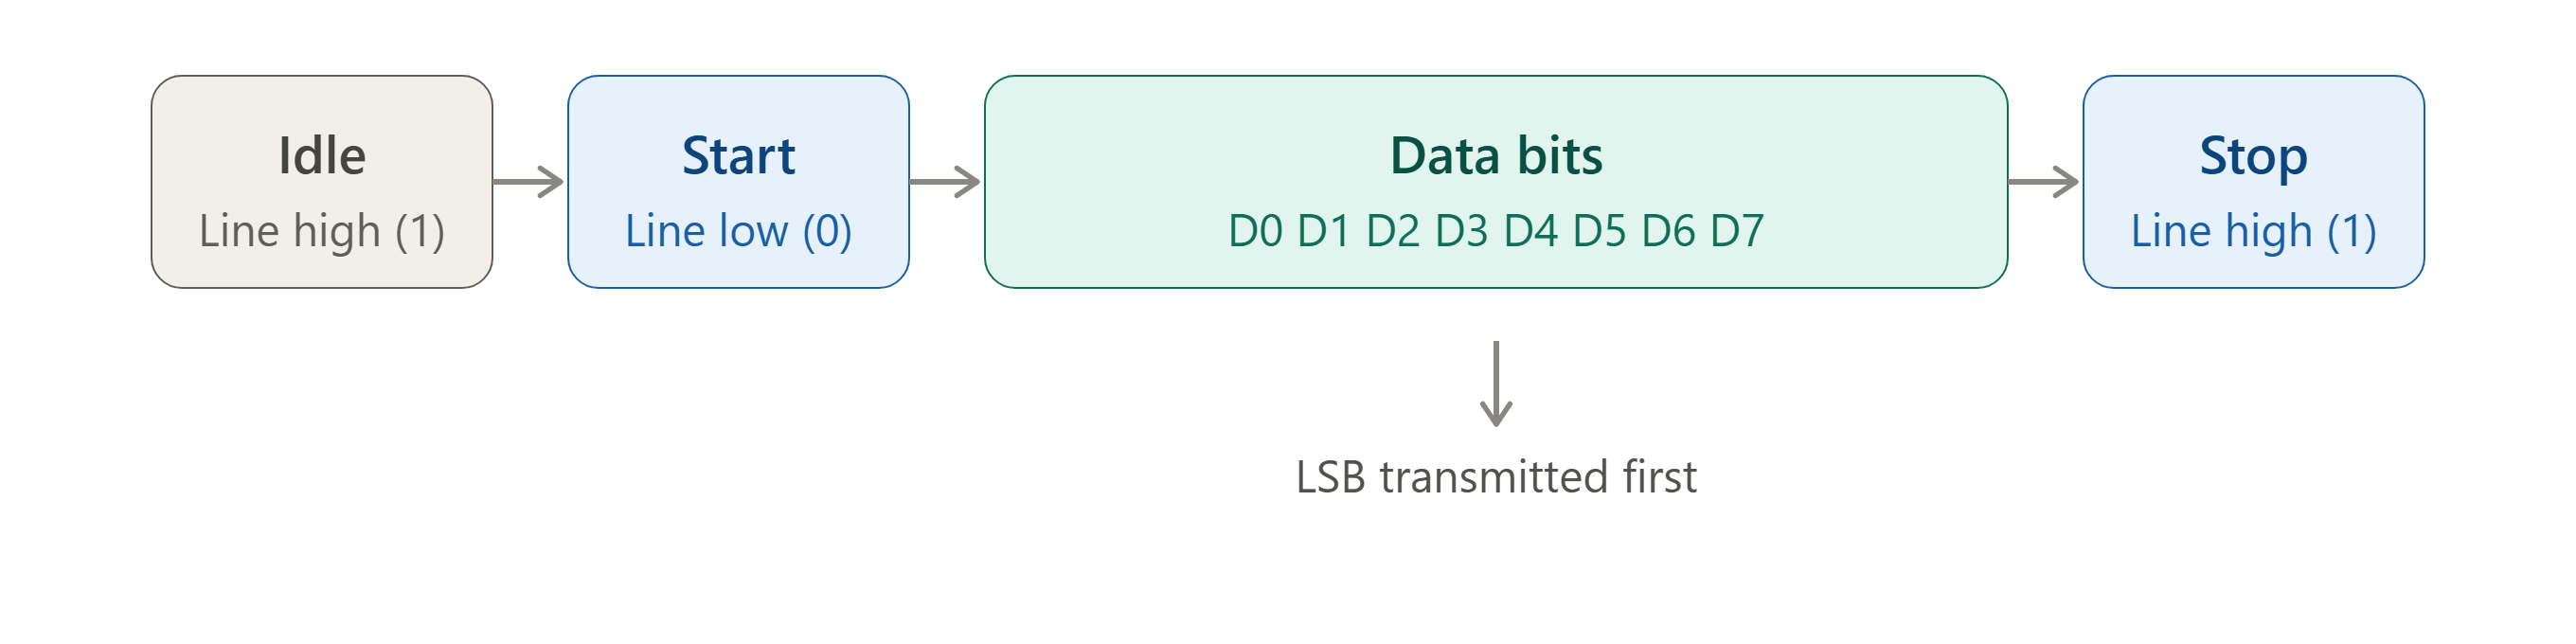
\includegraphics[width=0.90\linewidth]{images/uart_frame_flowchart.png}
    \caption{Standard UART Communication Frame.}
    \label{fig:uart_frame}
\end{figure}

Figure~\ref{fig:uart_frame} illustrates the structure of a standard UART data frame. Communication begins with a start bit followed by the data bits, an optional parity bit, and one or more stop bits. This frame structure enables asynchronous communication without requiring a dedicated clock signal between communicating devices.

%==========================================================

\section{Applications of UART}

Because of its simplicity and reliability, UART is widely employed in both academic and industrial electronic systems. Some common applications include:

\begin{itemize}

\item Embedded systems and microcontrollers

\item FPGA and ASIC-based digital systems

\item Sensor interfacing

\item GPS and Bluetooth communication modules

\item Industrial automation and control systems

\item Internet of Things (IoT) devices

\item Debugging and serial terminal communication

\item System-on-Chip (SoC) communication interfaces

\end{itemize}

The widespread adoption of UART makes it one of the most important communication peripherals in digital integrated circuits. Consequently, implementing a UART Transceiver IP Core using a complete RTL-to-GDSII ASIC design flow provides valuable practical experience in modern digital VLSI design methodologies.

\clearpage

%==========================================================

\section{Project Overview}

This project focuses on the complete RTL-to-GDSII implementation of 
a UART Transceiver IP Core using the OpenLane2 open-source ASIC design flow. The UART transceiver was designed in Verilog HDL and functionally verified using Verilator before proceeding through the complete physical implementation flow.

The implementation includes RTL design, functional verification, logic synthesis, floorplanning, power distribution network generation, placement, clock tree synthesis (CTS), global and detailed routing, parasitic extraction, static timing analysis (STA), IR-drop analysis, Design Rule Checking (DRC), Layout Versus Schematic (LVS) verification, and final GDSII layout generation. Throughout the implementation, reports generated at each stage were analyzed to evaluate design quality, area utilization, routing efficiency, timing performance, and manufacturability.

The project demonstrates how an RTL design is transformed into a fabrication-ready integrated circuit using an entirely open-source ASIC design environment based on the SkyWater SKY130A Process Design Kit (PDK).

%==========================================================

\section{Motivation}

Open-source Electronic Design Automation (EDA) tools have significantly simplified digital ASIC design by providing accessible alternatives to proprietary software. OpenLane2 integrates multiple open-source tools into a complete RTL-to-GDSII flow, enabling designers and students to gain practical experience in modern ASIC implementation.

The motivation behind this project is to understand every stage of the digital ASIC design flow by implementing a real communication IP core. Instead of limiting the work to RTL simulation, this project emphasizes complete physical implementation, report analysis, timing closure, routing optimization, physical verification, and manufacturability assessment.

%==========================================================

\section{Objectives}

The primary objectives of this project are:

\begin{itemize}

\item Design a synthesizable UART Transceiver IP Core using Verilog HDL.

\item Perform functional verification using Verilator.

\item Implement the complete RTL-to-GDSII ASIC flow using OpenLane2.

\item Analyze synthesis, placement, routing, timing, and utilization reports.

\item Perform RC extraction, IR-drop analysis, and static timing analysis.

\item Verify the final layout using Magic DRC, KLayout DRC, and Netgen LVS.

\item Generate a manufacturable GDSII layout.

\end{itemize}

%==========================================================

\section{Design Specifications}

Table~\ref{tab:design_specifications} summarizes the design environment and implementation specifications used throughout this project.

\begin{table}[!htbp]
\centering
\caption{Design Specifications}
\label{tab:design_specifications}

\renewcommand{\arraystretch}{1.3}

\begin{tabular}{|p{6cm}|p{7cm}|}
\hline

\textbf{Parameter} & \textbf{Specification} \\

\hline

Design & UART Transceiver IP Core \\

\hline

Hardware Description Language & Verilog HDL \\

\hline

Technology Node & 130 nm CMOS \\

\hline

Process Design Kit & SKY130A PDK \\

\hline

ASIC Flow & OpenLane2 \\

\hline

RTL Verification & Verilator \\

\hline

Logic Synthesis & Yosys \\

\hline

Physical Design & OpenROAD \\

\hline

Physical Verification & Magic, KLayout, Netgen \\

\hline

Operating System & Ubuntu 24.04 (WSL2) \\

\hline

Final Output & GDSII Layout \\

\hline

\end{tabular}

\end{table}

%==========================================================

\section{Project Methodology}

The complete implementation follows a standard digital ASIC design methodology beginning with RTL design and ending with GDSII generation. Each implementation stage produces reports that are analyzed to evaluate timing performance, silicon area, routing quality, power integrity, and physical correctness.

\begin{figure}[!htbp]
    \centering
    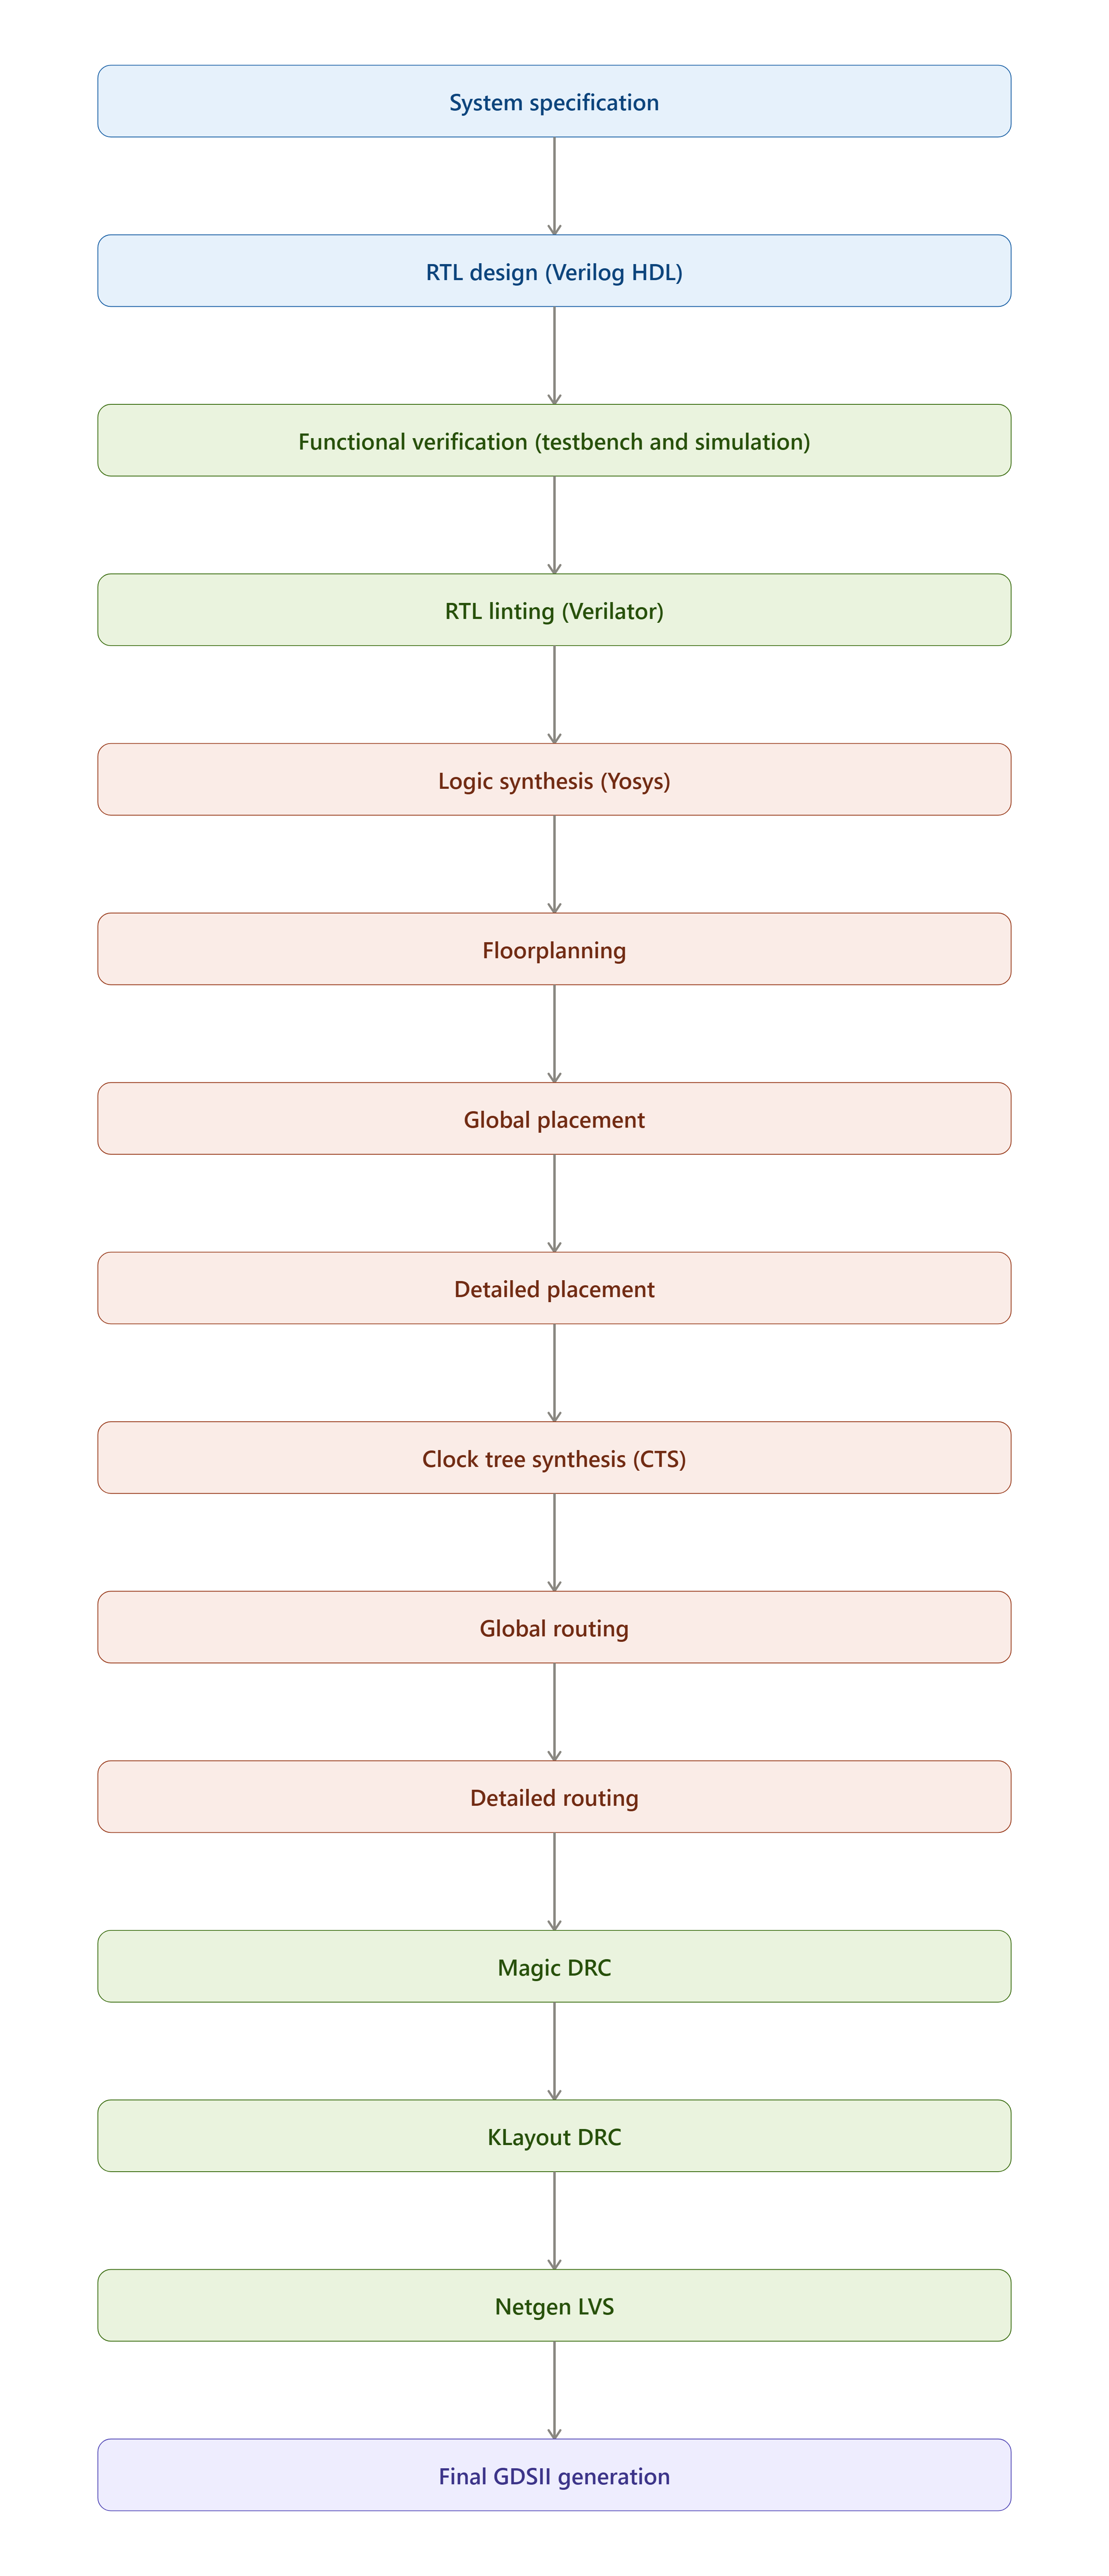
\includegraphics[width=0.92\linewidth]{images/asic_design_flow_full.png}
    \caption{Complete RTL-to-GDSII ASIC Design Flow adopted in this project.}
    \label{fig:asic_design_flow}
\end{figure}

As illustrated in Figure~\ref{fig:asic_design_flow}, the implementation begins with RTL development and functional verification, followed by logic synthesis, floorplanning, placement, clock tree synthesis, routing, RC extraction, static timing analysis, physical verification, and final GDSII layout generation. Each stage contributes to the successful realization of a fabrication-ready UART Transceiver ASIC.

The subsequent chapters discuss each implementation stage in detail, including the UART architecture, RTL implementation, verification methodology, physical design, report analysis, and signoff verification.

\clearpage